%%% Local Variables:
%%% mode: latex
%%% TeX-master: "../frankfurt"
%%% End:

\subsection{}
\begin{frame}
  \frametitle{Karger's Algorithm}
\only<1>{
      \begin{itemize}
    \item Contraction method is used.
      \item Randomized selection of Edges.
        \item Running multiple times of the algorithm will provide
          more accurate result.
    \end{itemize}
}

\only<2>{
  \begin{itemize}
\item Basically one run of Karger's Algo takes {\bf $O(n^2)$} time;
\item One time running the algorithm will make errors at the
  probability of  $O(\frac{1}{n^2})$;
\item Higher accuracy can be achieved by running the algorithm
  multiple times;
\item It achieves error probability of $\frac{1}{poly(n)}$ with
  $O(n^4\log{}n)$ time.
  \end{itemize}


}
\only<3>{

  \begin{itemize}
  \item Improved Karger's algorithm was developed by Karger and Stein;
  \item Achieving $O(n^2\log^3{n})$ running time;
  \item $O(\frac{1}{n})$ error probability.
  \end{itemize}
Derivation will be given in the later part.
}

\only<4>{

  \begin{block}{Comparison}
    \begin{itemize}
    \item A trivial algorithm checks all x {\bf \large TODO} possible subsets of $V$ and
      computes the weight of the resulting cuts, which takes {\bf
        \large TODO} time in total.
    \item Another algorithm({\bf\large TODO} the one that's based on
      many max-flow-computation) takes {\bf\large TODO} time.
    \end{itemize}
  \end{block}
 Well that's a lot of TODOS
}
\end{frame}


\begin{frame}
  \frametitle{Algorithm}
\only<1>{

\begin{greenblock}{Karger's Algorithm:}
      \begin{algorithm}[H]
        \small
        \Repeat{G has 2 vertices}{
          {\bf choose} an edge $(v, w)$ uniformly at random from G\;
          {\bf let} $G\leftarrow \frac{G}{(v,w)}$
        }
        % \caption{Descent Method Algorithm}
      \end{algorithm}
    \end{greenblock}

}

\only<2>{
\hspace*{1.8cm}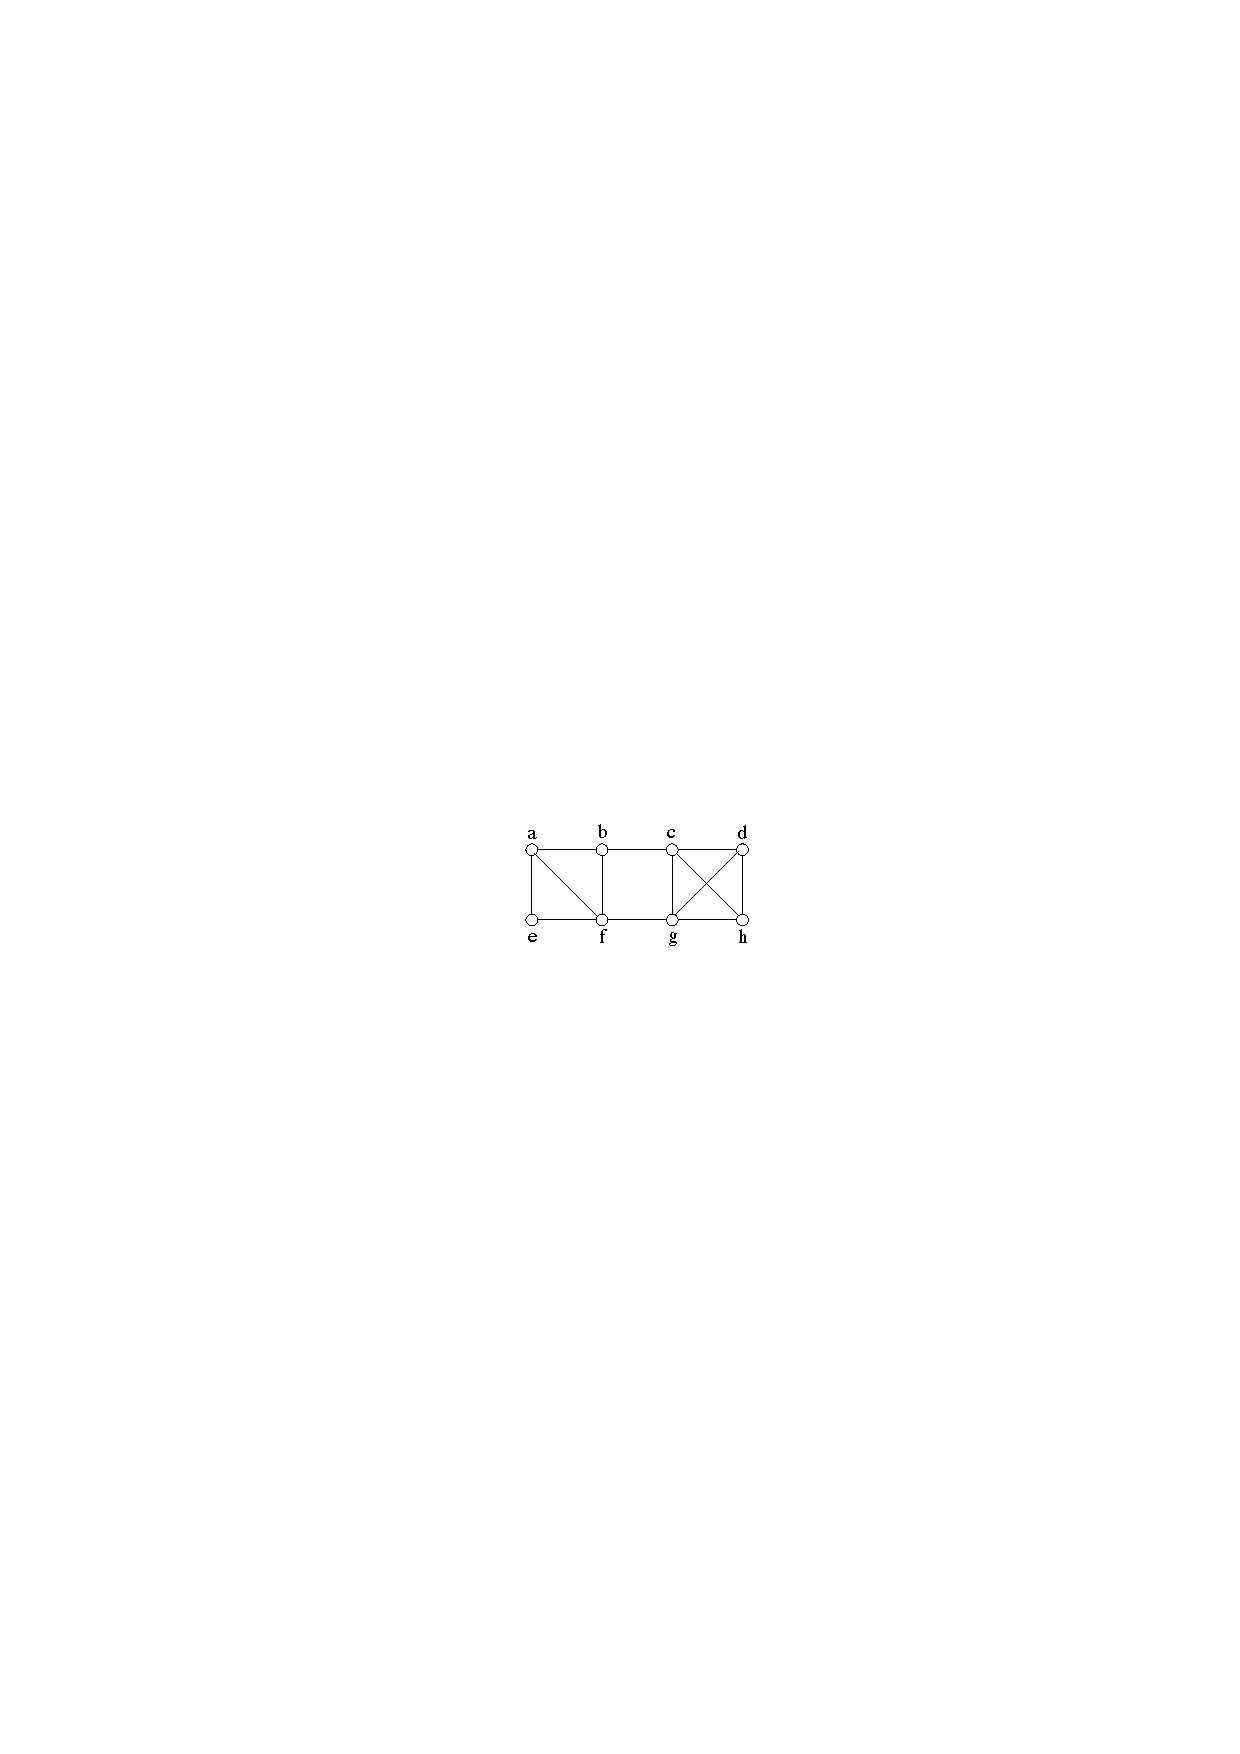
\includegraphics[scale=1.7]{img/examplegraph_modified.pdf}

}
\only<3>{
\hspace*{1.8cm}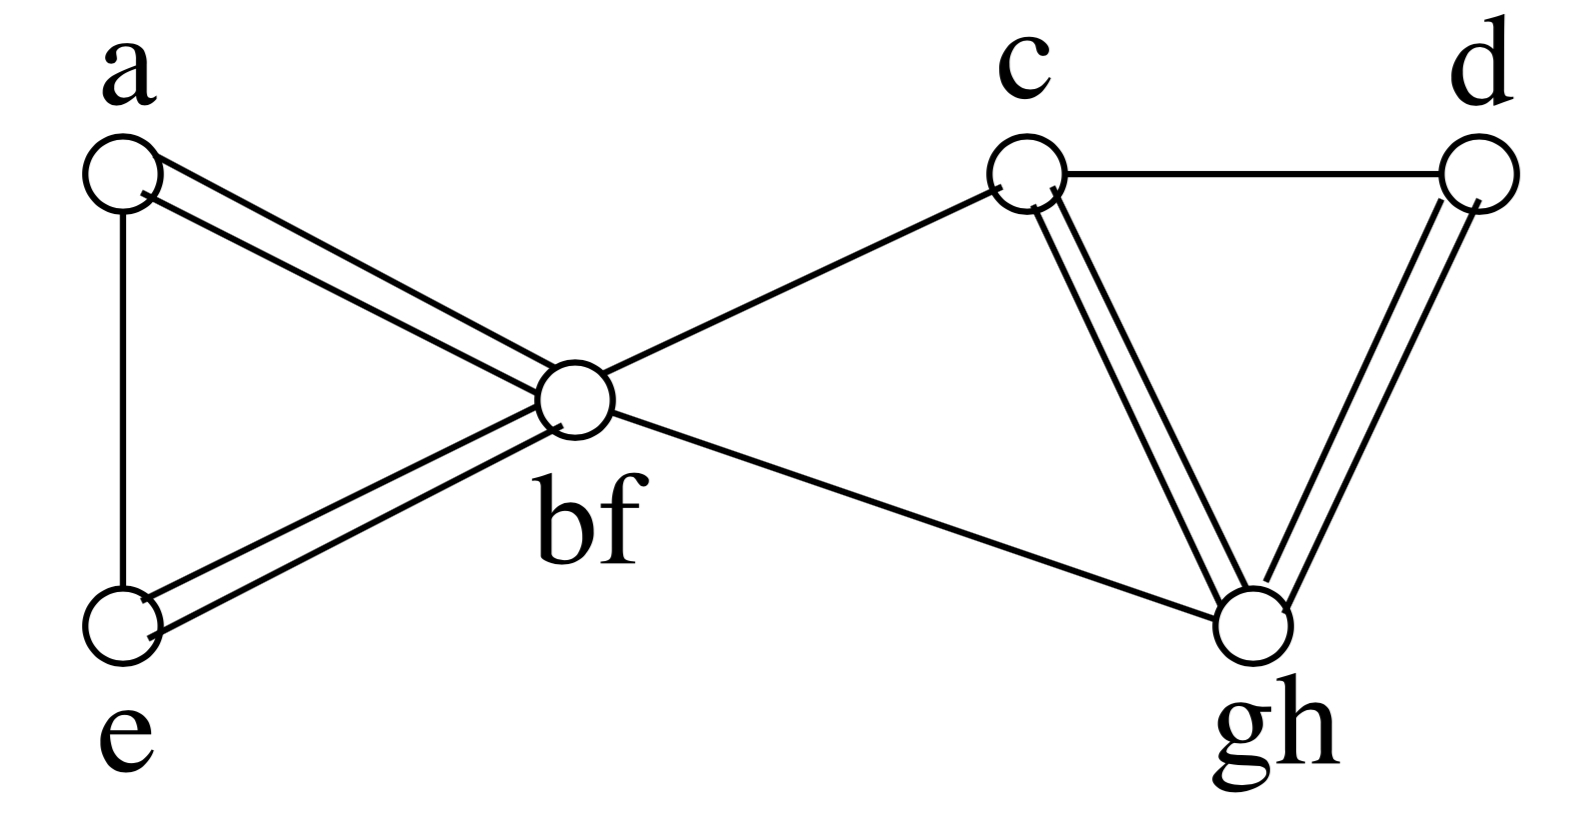
\includegraphics[scale=0.2]{img/2.png}

}
\only<4>{
\hspace*{1.8cm}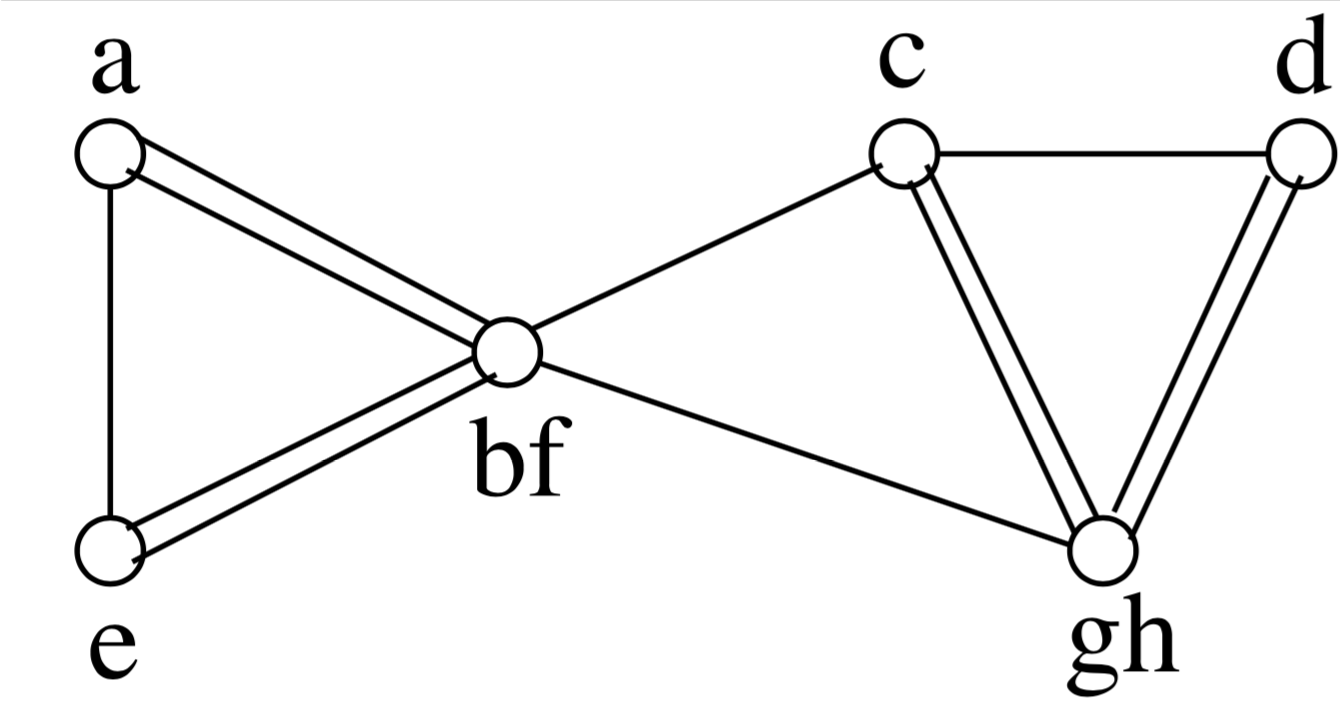
\includegraphics[scale=0.2]{img/3.png}

}
\only<5>{
\hspace*{1.8cm}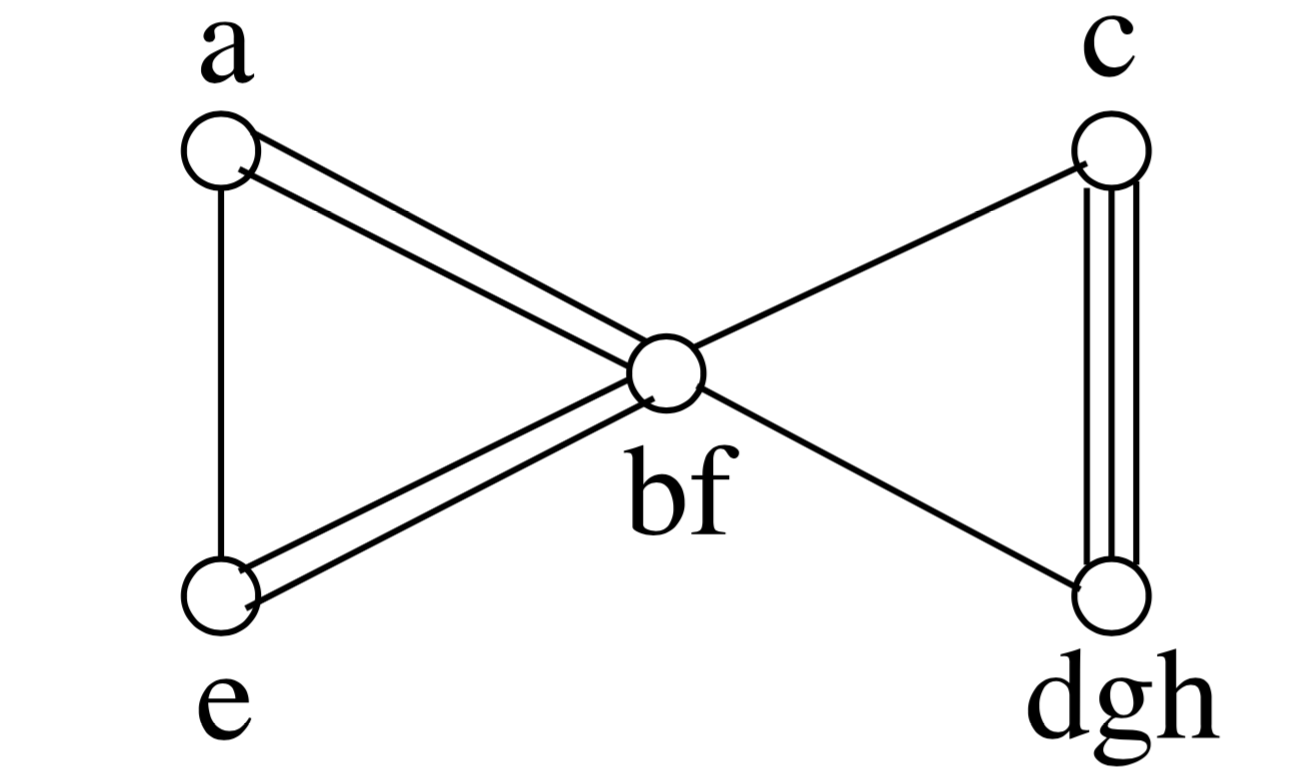
\includegraphics[scale=0.2]{img/4.png}

}
\only<6>{
\hspace*{1.8cm}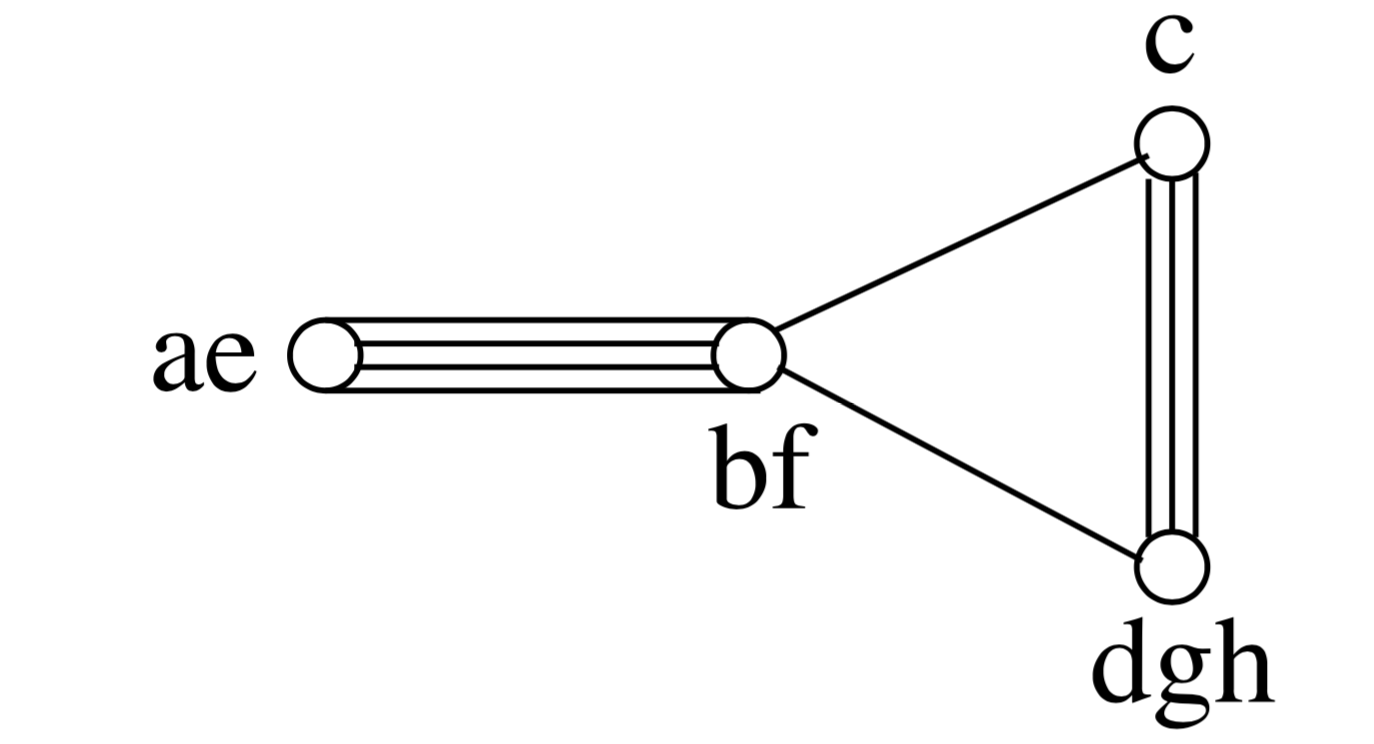
\includegraphics[scale=0.2]{img/5.png}

}
\only<7>{
\hspace*{1.8cm}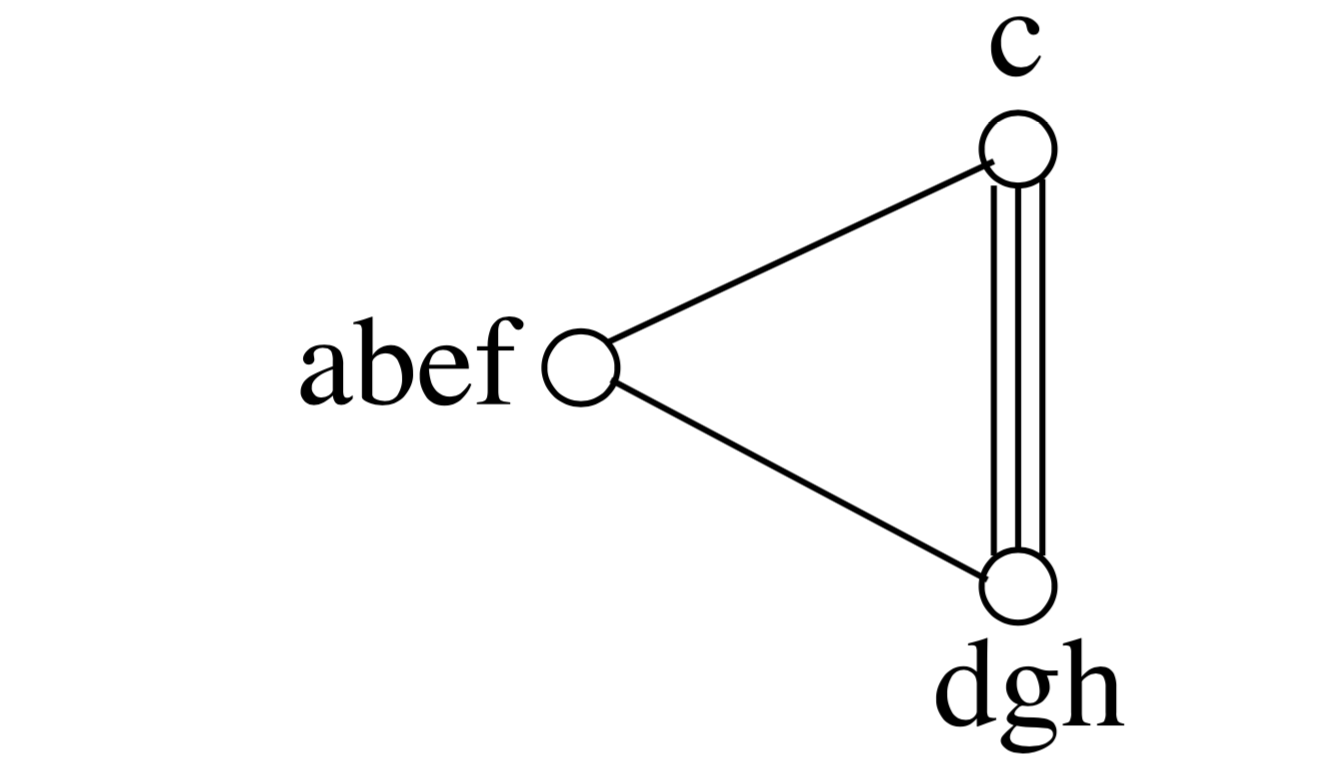
\includegraphics[scale=0.2]{img/6.png}
}

\only<8>{
\hspace*{1.8cm}
\includegraphics[scale=0.2]{img/7.png}
}

% http://www.cs.berkeley.edu/~jordan/courses/174-spring02/recitation/lec5.pdf
\end{frame}

\begin{frame}
  \frametitle{Results}

\vspace*{-1.5cm}
  \hspace*{2cm}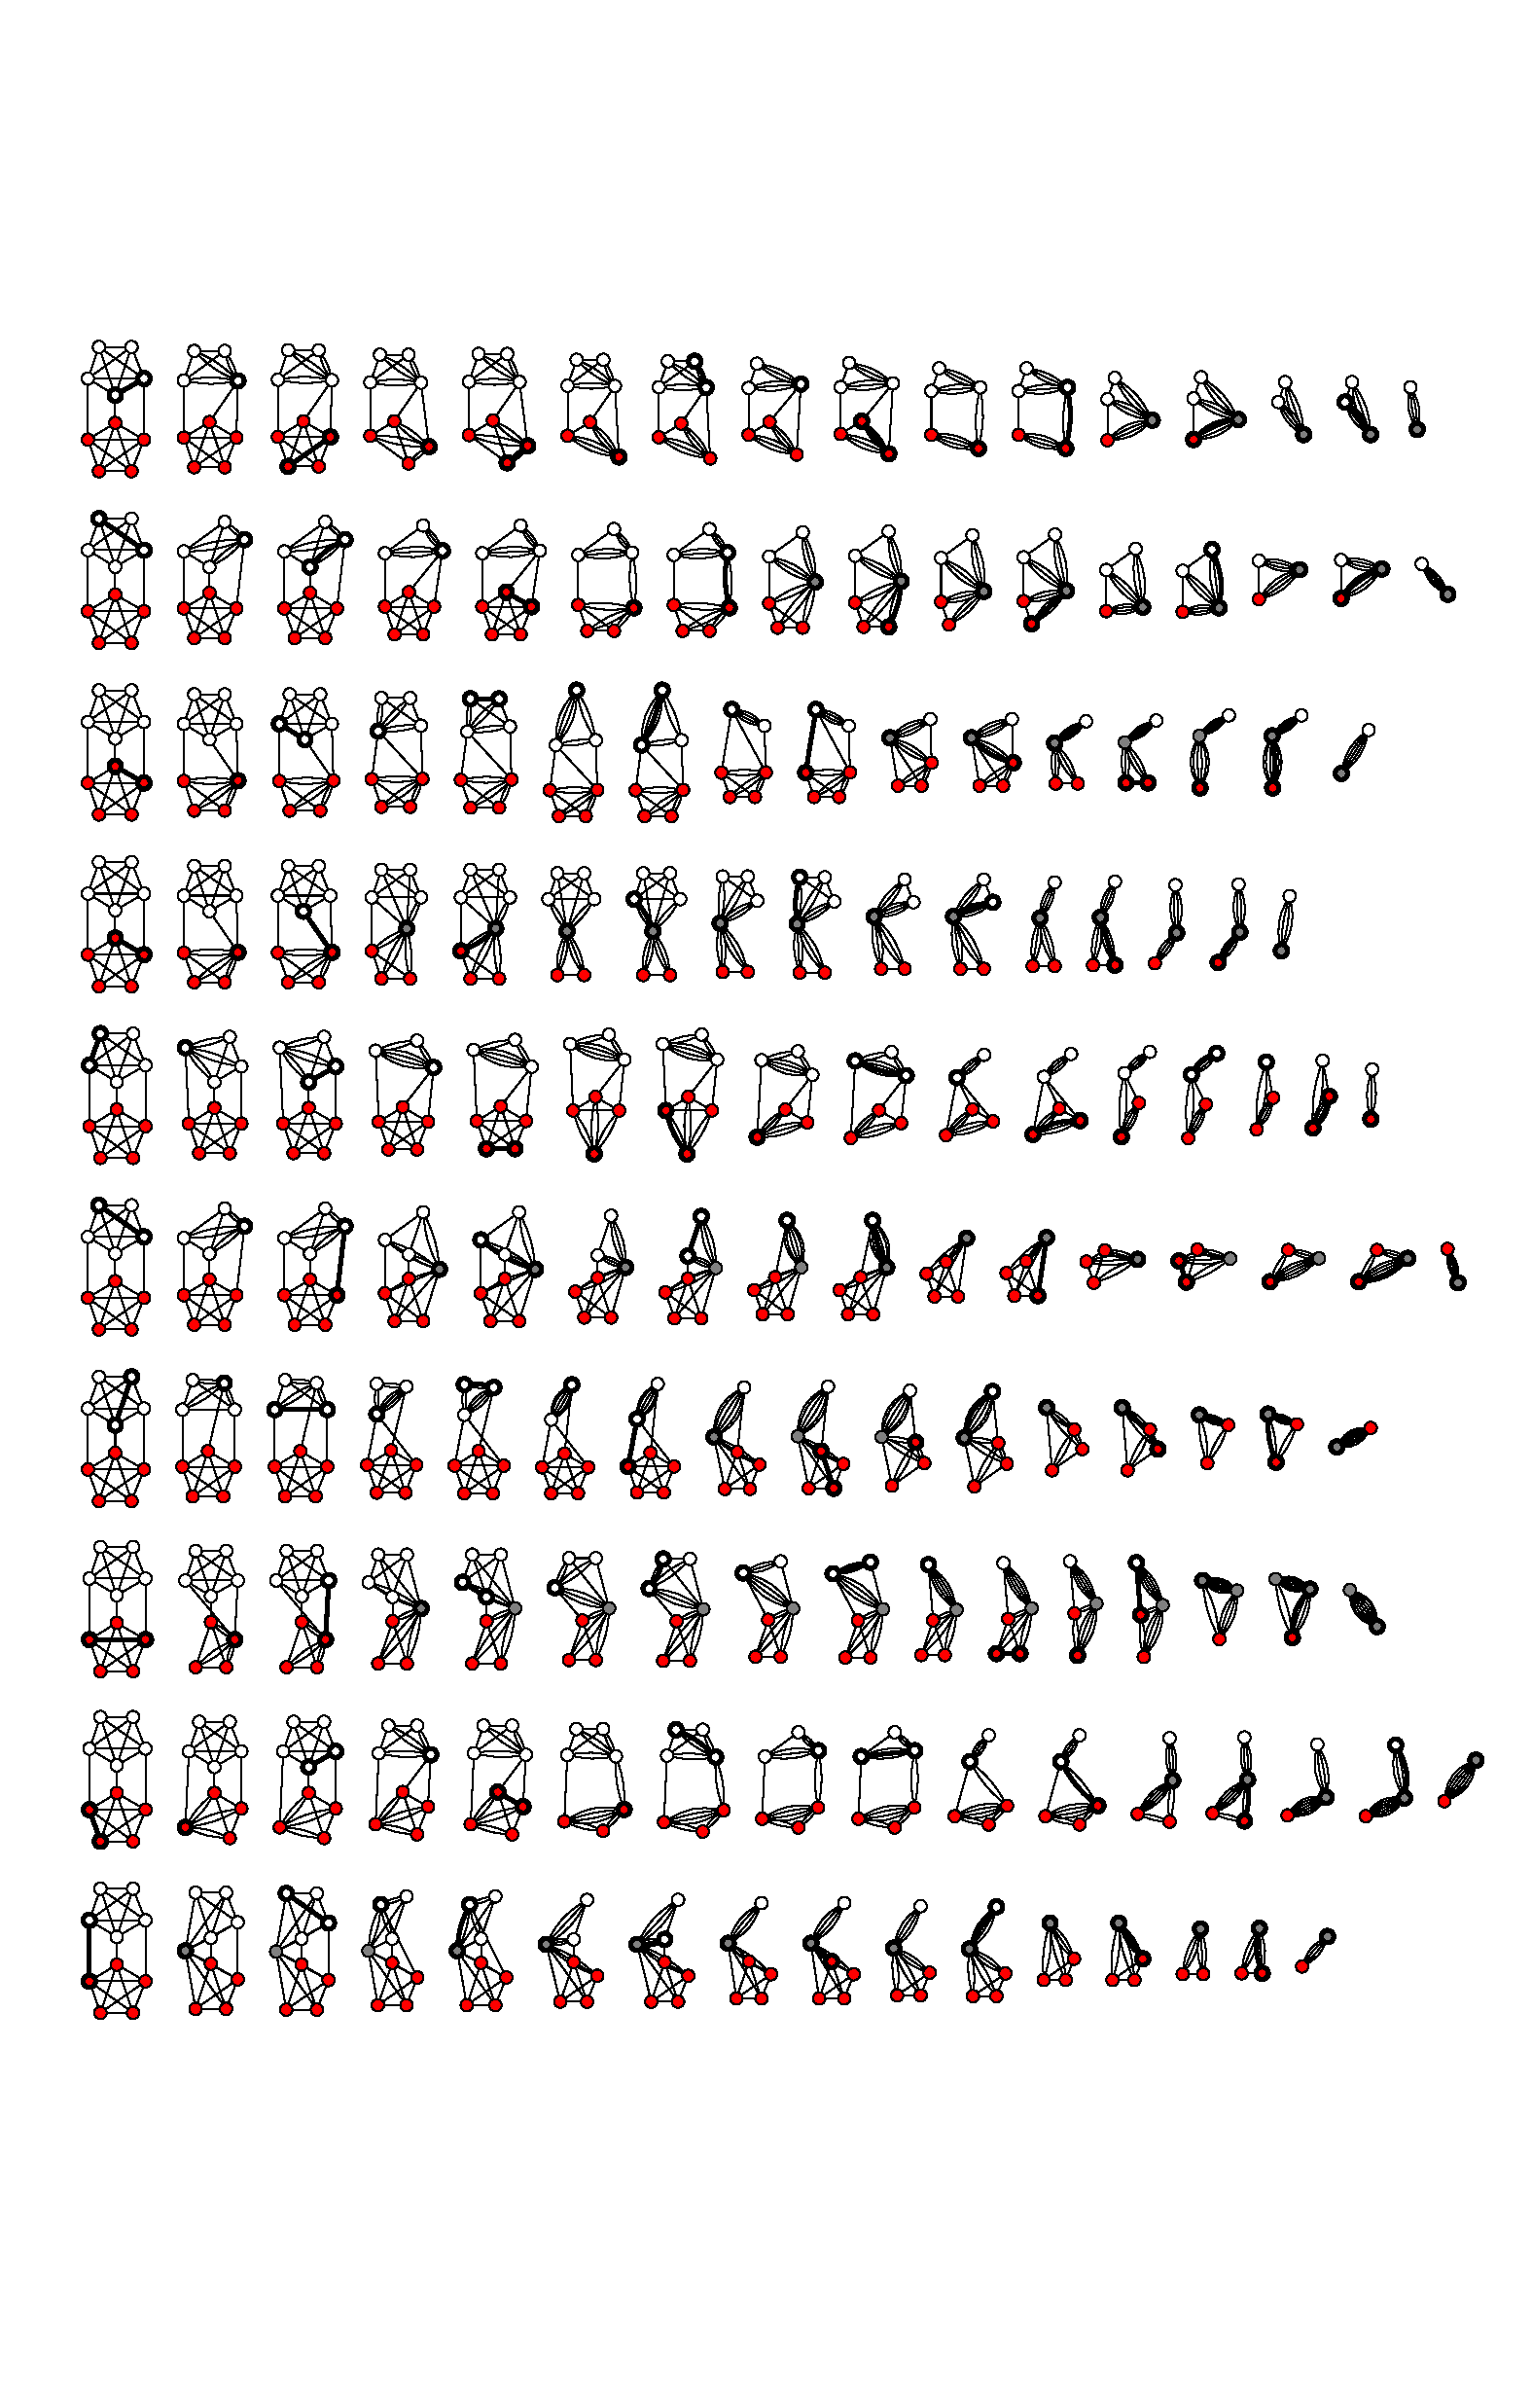
\includegraphics[scale=0.25]{img/kargers.pdf}
\end{frame}
